\documentclass[14pt, a4paper]{book}
\usepackage[utf8]{inputenc}
\usepackage[T1]{fontenc}
\usepackage[margin=1in,marginpar=0.9in]{geometry} 
\usepackage{amsmath,amsthm,amssymb,amsfonts, fancyhdr, color, comment, graphicx, environ, bm}
%\usepackage{xcolor}
%\usepackage{mdframed}
\usepackage[shortlabels]{enumitem}
% \usepackage[american]{duomasterforside}
\usepackage[USenglish]{uiomasterfp}
%\usepackage{indentfirst}
%\usepackage{simpler-wick}
\usepackage{booktabs}
%\usepackage{siunitx}
\usepackage{physics}
%\usepackage{polynom}
%\usepackage{verbatim}
%\usepackage{tensor}
\usepackage{todonotes}
\usepackage{slashed}
%\usepackage{dcolumn}% Align table columns on decimal point
\usepackage{listings}
\renewcommand{\lstlistingname}{Algorithm}
\usepackage{caption}
\usepackage{subcaption}
\usepackage[backend = biber, style = vancouver]{biblatex}
\usepackage{biblatex}
\usepackage[printonlyused,withpage]{acronym}
\addbibresource{refs.bib}
\usepackage{hyperref}
\hypersetup{
    colorlinks=true,
    linkcolor=blue,
    filecolor=magenta,      
    urlcolor=cyan,
    citecolor=cyan,
    pdftitle={Model\_independent\_search\_for\_Dark\_Matter\_using\_Machine\_Learning},
    pdfpagemode=FullScreen,
    }
\usepackage{tikz}
\tikzset{every picture/.style={line width=0.75pt}} %set default line width to 0.75pt

\definecolor{codegreen}{rgb}{0,0.6,0}
\definecolor{codegray}{rgb}{0.5,0.5,0.5}
\definecolor{codepurple}{rgb}{0.58,0,0.82}
\definecolor{backcolour}{rgb}{0.95,0.95,0.92}

\lstdefinestyle{mystyle}{
	backgroundcolor=\color{backcolour},   
	commentstyle=\color{codegreen},
	keywordstyle=\color{magenta},
	numberstyle=\tiny\color{codegray},
	stringstyle=\color{codepurple},
	basicstyle=\ttfamily\footnotesize,
	breakatwhitespace=false,         
	breaklines=true,                 
	captionpos=b,                    
	keepspaces=true,                 
	numbers=left,                    
	numbersep=5pt,                  
	showspaces=false,                
	showstringspaces=false,
	showtabs=false,                  
	tabsize=2
}
\lstset{style=mystyle}
\usepackage{subfiles} 


\title{Model independent search for Dark Matter using Machine Learning 
with dilepton and Missing Transverse Energy final states with the ATLAS detector at the LHC 
}
\author{Ruben Guevara}
\date{Spring 2023}

\begin{document}
\pagenumbering{roman}

% \duoforside[
% dept = {Department of Physics},
% long,
% program = {Physics: Nuclear and Particle Physics},
% ]

\uiomasterfp[
colour = pink,
dept = {Department of Physics},
long,
program = {Physics: Nuclear and Particle Physics},
supervisors = {Professor Farid Ould-Saada \and Dr. Eirik Gramstad}
]
\newpage
\section*{Acknowledgements}
Thank you everybody<3<3

\newpage
\begin{center}
\section*{Abstract}
Something something
\end{center}


\newpage
\tableofcontents
\listoffigures
\listoftables

\chapter*{List of Acronyms}
\textbf{SM} Standard Model\\\\
\textbf{DM} Dark Matter\\\\
\textbf{LHC} Large Hadron Collider\\\\
\textbf{MET} Missing Transverse Energy\\\\
\textbf{ML} Machine Learning\\\\
\textbf{NN} Neural Network\\\\
\textbf{BDT} Bosted Decision Tree\\\\
\newpage
\pagenumbering{arabic}


\part{The theory behind modern particle physics / Background}


\chapter{The Standard Model of Particle Physics}
\subfile{chapters/Part_I/1_The_Standard_Model_of_Particle_Physics.tex}



\chapter{Dark Matter}
\subfile{chapters/Part_I/2_Dark_Matter.tex}




\chapter{Production, Detection and Analysis}
\subfile{chapters/Part_I/3_Production_Detection_and_Analysis.tex}


\chapter{Machine Learning}
\subfile{chapters/Part_I/4_Machine_Learning.tex}

\part{Implementation / Methods}
\chapter{Data Analysis}
\subfile{chapters/Part_II/5_Data_Analysis.tex}

\chapter{Machine Learning}\label{chap:ML}
\subfile{chapters/Part_II/6_Machine_Learning.tex}

\part{Results}

\graphicspath{{figures/}}
% \graphicspath{{../../figures/}}

\chapter{Comparison to cut and count}
Testing three models using the classical data analysis way we apply cuts to kinematic variables and try to isolate the signal from the background to then calculated the expected significance. The three models I chose to test are all High Dark Sector models with $m_{Z'}=130$GeV. They are a Light Vector (LV), Dark Higgs (DH) and Effective Field Theory (EFT) models. The cuts I made on these are shown in Table \ref{tab:cuts}.
\begin{table}[!h]
    \centering
    \begin{tabular}{l|r}\midrule\midrule
                                & Cut\\\midrule
         $E_T^{miss}/\sigma$    & > 10      \\
         $m_T$                  & > 160 GeV \\
         $m_{ll}$               & > 120 GeV \\
         Number of B-jets       & 0         \\
         $m_{T2}$               & > 110 GeV \\\midrule\midrule
    \end{tabular}
    \caption[Cut and count cuts]{Table showcasing the cuts used when doing the cut and count method.}
    \label{tab:cuts}
\end{table}
\\ Since the cross section to find Dark Matter is really small we have to use the low-statistics expected significance formula to find the closest to correct significance. The formula is
\begin{equation}\label{eq:low_stat_Z}
    Z = \sqrt{2\left[(s + b)\ln(1 + \frac{s}{b}) - s \right]}
\end{equation}
Where $s$ is the number of signal events and $b$ is the number of background events. Using this we get the results shown in Table \ref{tab:cutsigee} for the electron channel and Table \ref{tab:cutsiguu} for the muon channel. Also included on the tables are the number of events. One thing worth mentioning is that when adding another cut on the maximum invariant mass increases the significance. The significance for LV on the electron channel was at $1.2\sigma$ when adding a cut stating that $m_{ll}<150$ GeV. This makes sense since the models in question all have a $m_{Z'}=130$GeV. This cut was not added since we do not want to put a cap on the mass of the propagator, as we don't know what the real mass is.
\begin{table}[!h]
    \centering
    \begin{tabular}{l|c|c|c|r}\midrule\midrule
                                          & LV  & DH  & EFT & Background \\\midrule
         Events before cuts               & 15  & 20  & 0   & 1,256,624    \\
         Events after cuts                & 4   & 6   & 0   & 117 \\
         Expected significance [$\sigma$] & 0.4 & 0.6 & 0   & \\\midrule\midrule
    \end{tabular}
    \caption[Cut and count significance ee]{Table showcasing the result of the cut and count method for the electron channel.}
    \label{tab:cutsigee}
\end{table}
\begin{table}[!h]
    \centering
    \begin{tabular}{l|c|c|c|r}\midrule\midrule
                                          & LV  & DH  & EFT & Background \\\midrule
         Events before cuts               & 14  & 19  & 0   & 1,626,098    \\
         Events after cuts                & 3   & 5   & 0   & 108 \\
         Expected significance [$\sigma$] & 0.36 & 0.51 & 0   & \\\midrule\midrule
    \end{tabular}
    \caption[Cut and count significance uu]{Table showcasing the result of the cut and count method for the muon channel.}
    \label{tab:cutsiguu}
\end{table}
\\If we were to compare these results with what our NN and BDT that trained on the full dataset we see that we can calculate the expected significance in different locations for the validation plots. Testing on the networks that trained using the data scientist method on the full DM dataset we get the results shown in Figure \ref{fig:XGB_SIG_FULL} for XGBoost and Figure \ref{fig:NN_SIG_FULL} for the Neural Network.
\begin{figure}[!ht]
	\centering
	\begin{subfigure}[b]{0.8\textwidth}
        \centering
        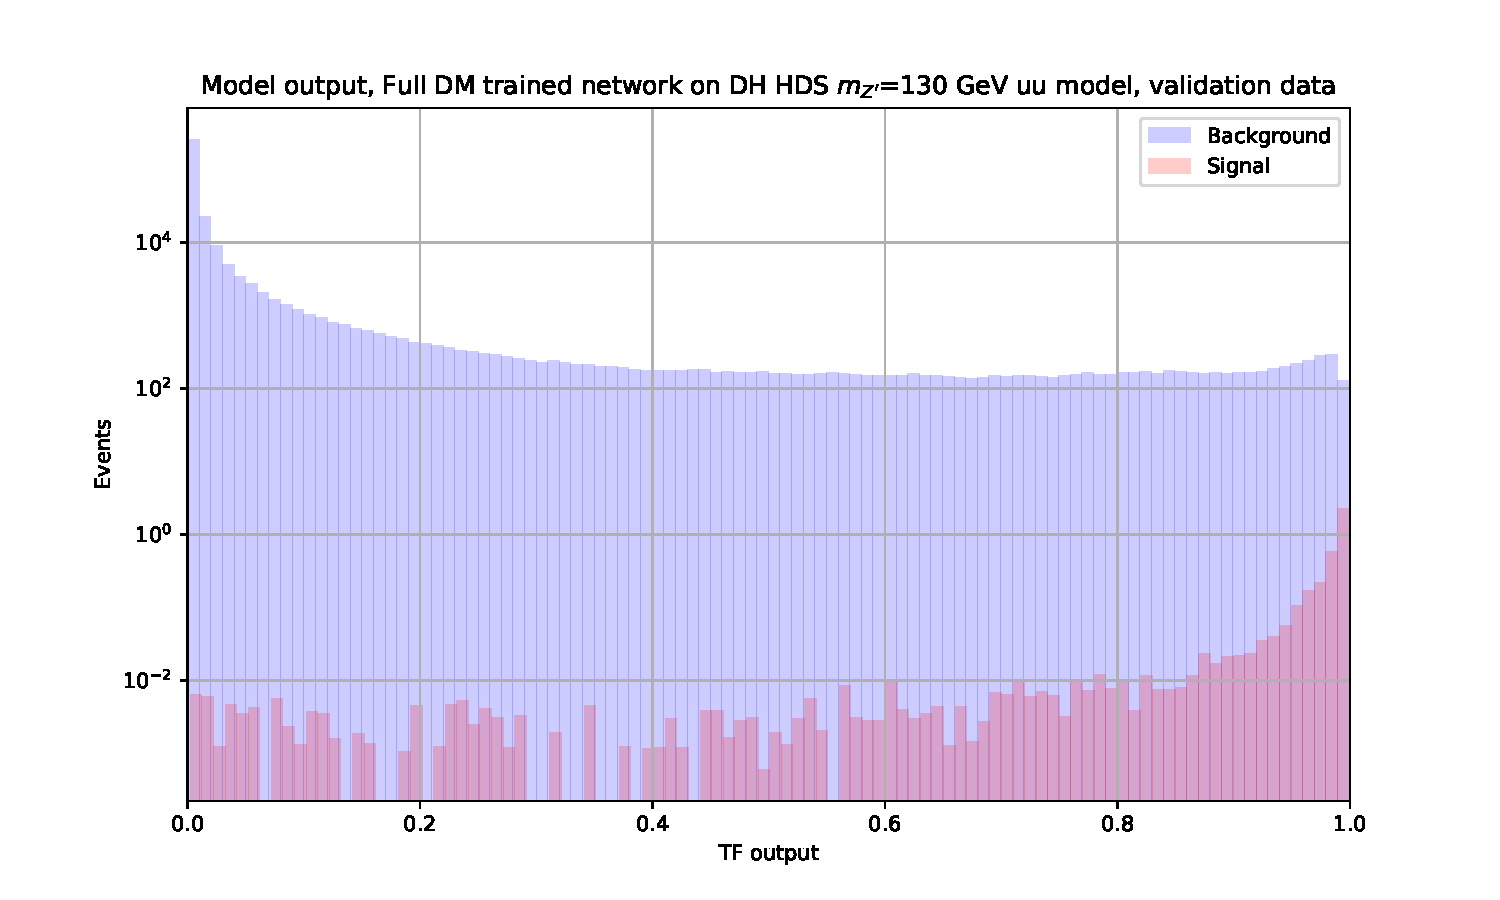
\includegraphics[width=1\textwidth]{XGB_VAL_uu.pdf}
        \caption{Validation plot.}\label{fig:XGB_VAL_UU}
     \end{subfigure}
     \hfill
     \begin{subfigure}[b]{0.8\textwidth}
        \centering
        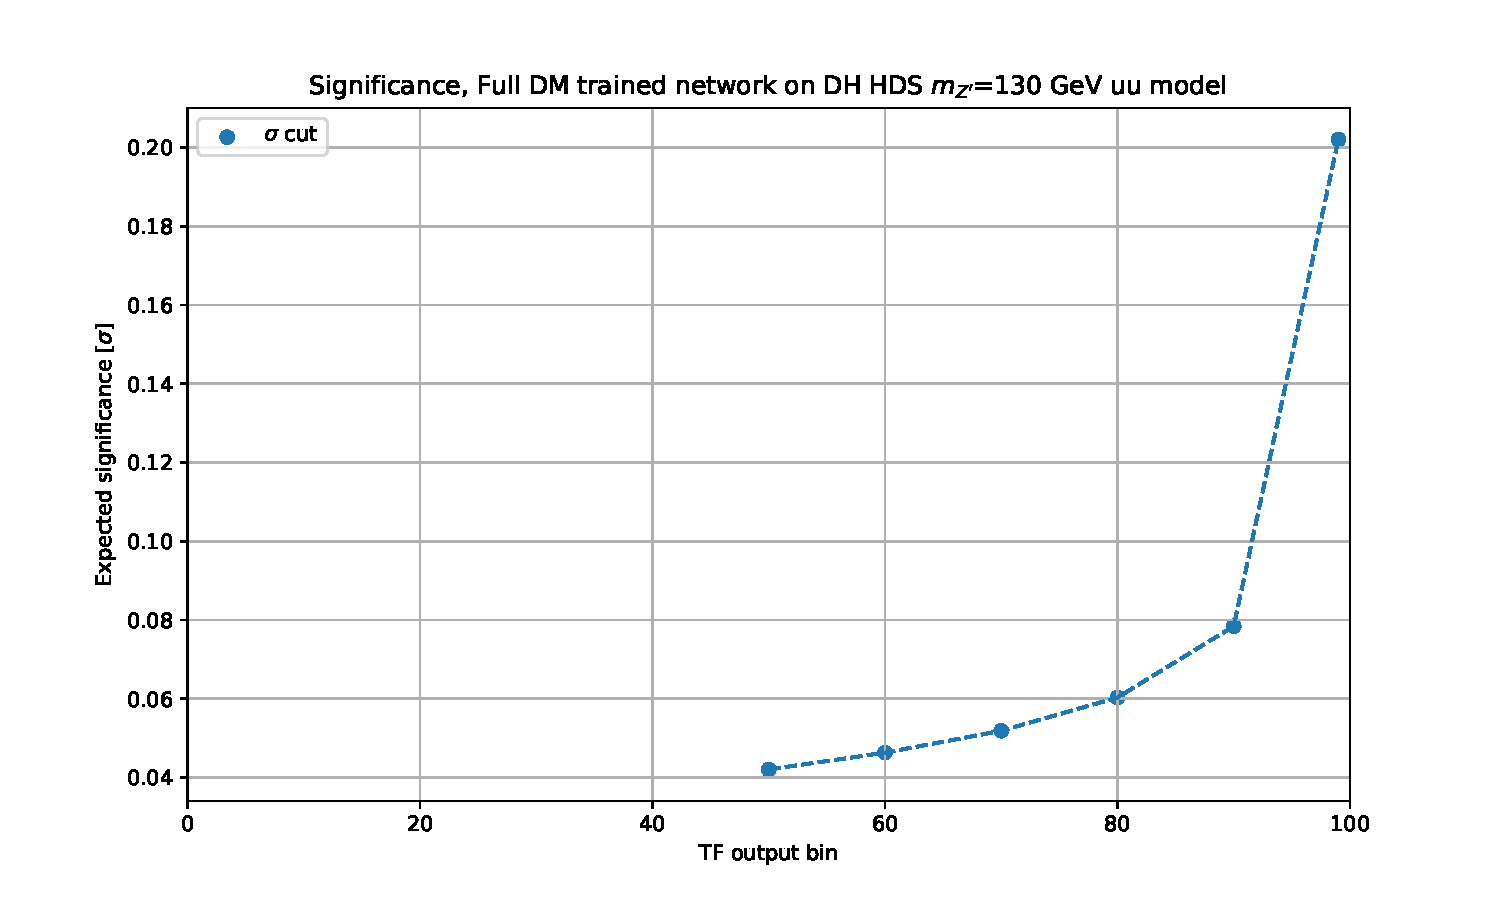
\includegraphics[width=1\textwidth]{XGB_EXP_SIG_uu.pdf}
        \caption{Expected significance when looking at bins and forth.}\label{fig:XGB_EXP_SIG:uu}
     \end{subfigure}
	\caption{Expected significance of XGBoost when trained on the Full DM dataset for the DH HDS $m_{Z'}$ = 130 GeV muon model.}\label{fig:XGB_SIG_FULL}
\end{figure}
\begin{figure}[!ht]
	\centering
	\begin{subfigure}[b]{0.8\textwidth}
        \centering
        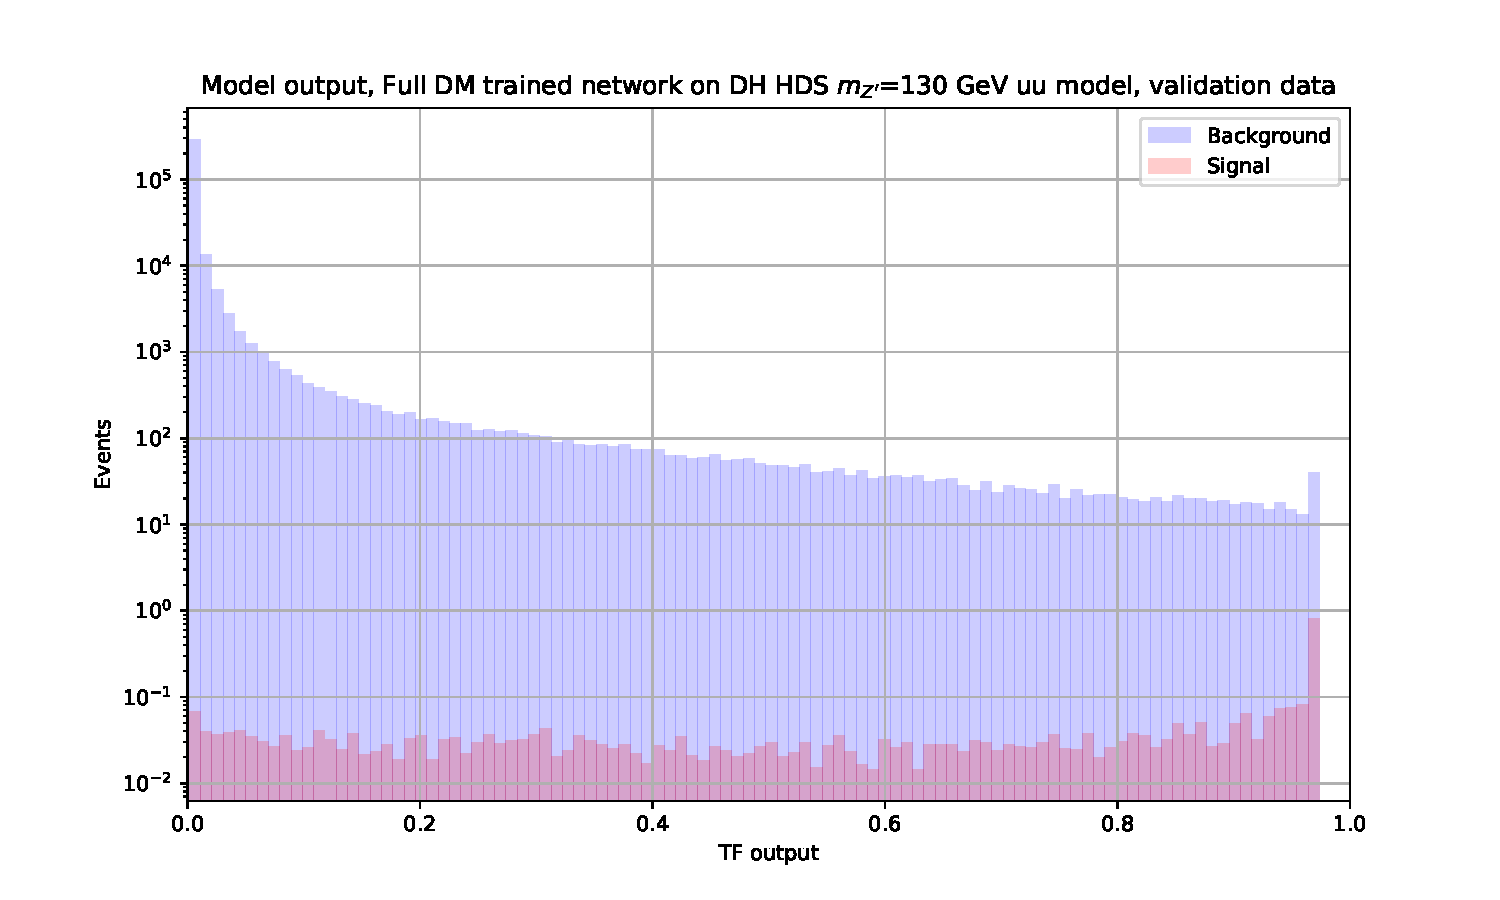
\includegraphics[width=1\textwidth]{NN_VAL_uu.pdf}
        \caption{Validation plot.}\label{fig:NN_VAL_UU}
     \end{subfigure}
     \hfill
     \begin{subfigure}[b]{0.8\textwidth}
        \centering
        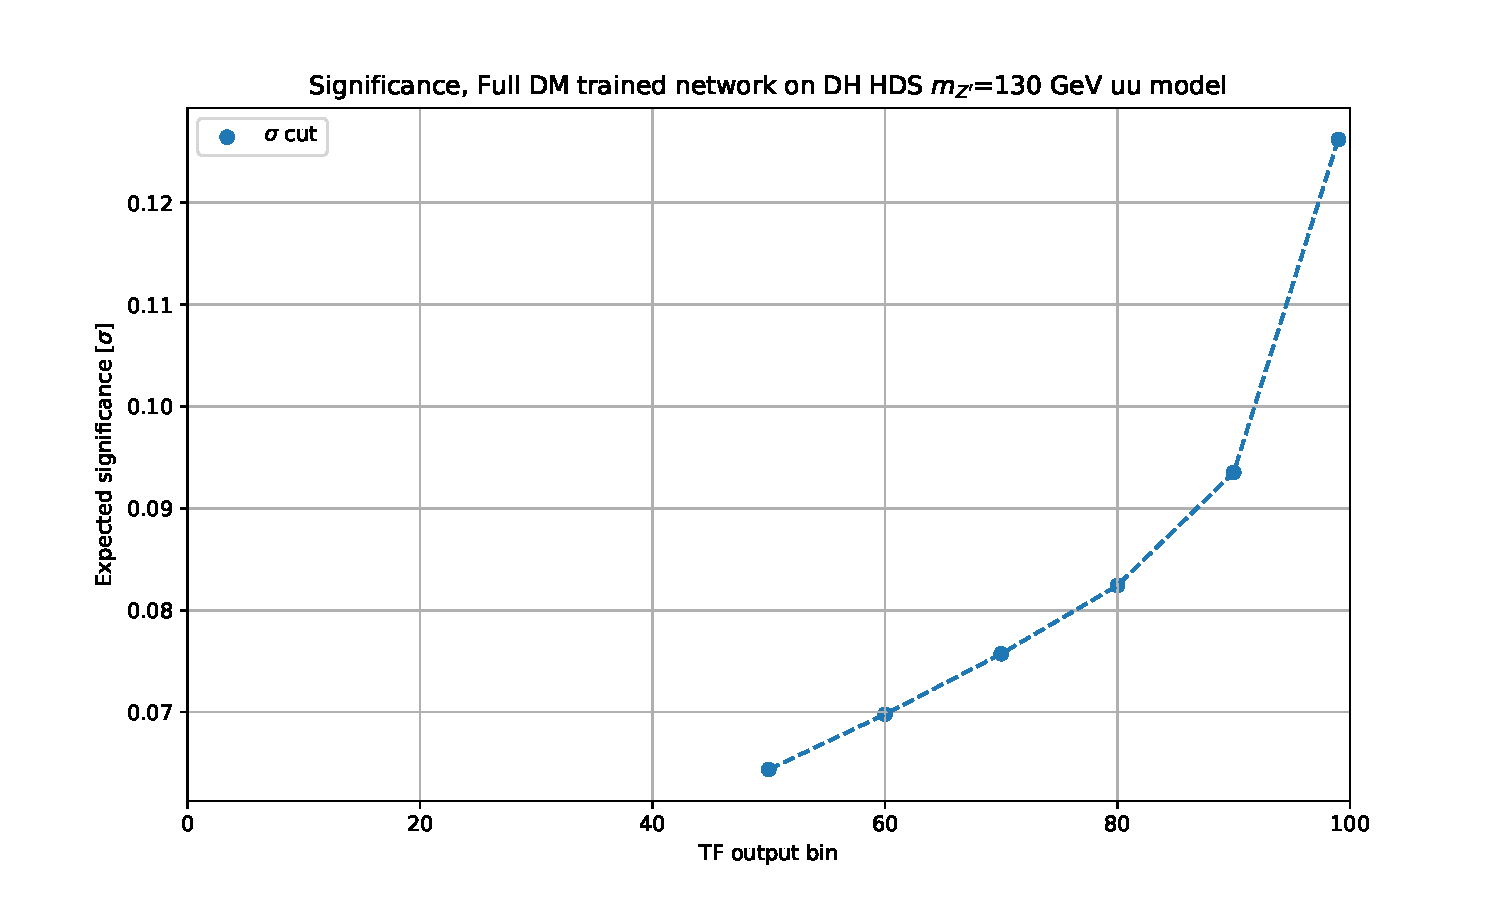
\includegraphics[width=1\textwidth]{NN_EXP_SIG_uu.pdf}
        \caption{Expected significance when looking at bins and forth.}\label{fig:NN_EXP_SIG:uu}
     \end{subfigure}
	\caption{Expected significance of the Neural Network when trained on the Full DM dataset for the DH HDS $m_{Z'}$ = 130 GeV muon model.}\label{fig:NN_SIG_FULL}
\end{figure}
\clearpage As we can see the expected significance is lower using ML than a rough cut and count. My theory for why this is the case is because we are testing just \textit{\textbf{one}} sample out of 154 different ones that are included for the three different theories I have acquired so far. And the ML networks shown above have both trained on a dataset including all 154 DM samples. The models that I tested might also not have been one of the "important" models the network learned from. Thus if I were to train the network individually based on the theory it might give better results.

\clearpage
\begin{table}[!h]
   \centering
   \begin{tabular}{l|c|c|c|r}\midrule\midrule
                                                & Signal     & Background \\\midrule
        MC events                               & 2,990,986  & 69,664,902 \\
        Sum of "Weight"                         & 388.75     & 2,714,091.3 \\
        Sum of generator weights                & 236.3      & 55,446,228,776,354.8 \\
        Sum of (generator weights*lumi / SOW)   & 9,167.1    & 61.1 \\
        Sum of (generator weights/SOW)          & 199.21    & 1.52 \\\midrule\midrule
   \end{tabular}
   \caption[Cut and count significance ee]{Table showcasing the result of the cut and count method for the electron channel.}
%    \label{tab:cutsigee}
\end{table}

\begin{table}[!h]
    \centering
    \begin{tabular}{l|c|c|c}\midrule\midrule
                    & Number of events & Sum of weights & Events $\times$ SOW [$10^{13}$]\\\midrule
         Signal     & 2,991,543        & 36,327,943.99  & 1.08\\
         Background & 69,664,345       & 36,327,944.03  & 25.3 \\ \midrule\midrule
    \end{tabular}
    \caption[Unbalanced DM training dataset]{Table Showcasing how uneven the training dataset is between signal and background. This is on the dataset which incorporates all the different DM MC samples}
    \label{tab:UnbalancedDMTraining}
\end{table}
in spacetime.
balance re-weighted bkg with raw MC signal. chatgpt was right about sample weights (its summed over though, keep that in mind)
\clearpage
\printbibliography

\end{document}
